\subsection{Estructura Interna del Servidor Spring Boot}
En la figura \ref{fig:DCG} se puede visualizar de manera general los componentes que conforman al servidor Java Spring Boot y el cómo se comunican.

Como punto de partida se tiene el paquete de los controladores (`com.example.PruebaCRUD.Controllers`). Estas clases son las encargadas de manejar las solicitudes HTTP que le llegan al servidor, así como de devolver una respuesta a dicha solicitud \cite{SpringController}. En otras palabras, estas clases son las encargadas de pasar la información entre la vista y el modelo. Para este caso en particular, estas clases se comunican con las clases de servicio, las cuales se encuentran en el paquete `com.example.PruebaCRUD.Services` y hacen uso de las clases que se encuentran en el paquete `com.example.PruebaCRUD.DTO`. 

Los DTO (Data Transfer Object), son clases que facilitan la transferencia de datos a través de la red o entre diferentes capas dentro del sistema \cite{DTO}. Como se puede ver dentro del diagrama, estos DTO son usados por la mayoría de las clases: las clases Controller, las cuales ya fueron descritas, así como las clases Service y Repository, de las cuales se explicarán a continuación.

Las clases de tipo Service son clases que se encargan de gestionar toda la lógica de negocio del sistema \cite{yadav-2024}. Funciona como intermediario entre los controladores y los repositorios.

Por otra parte, se encuentran los archivos de tipo Repository. Estos archivos son interfaces que permiten el acceso a la base de datos y el realizar operaciones CRUD \cite{diaz-2023}. Al extender de `JpaRepository`, estas interfaces heredan métodos para manipular entidades, eliminando la necesidad de implementar muchas de estas operaciones de manera manual.

Finalmente, se muestran a las clases de tipo Entity. Estas clases son parte de la capa de persistencia, y permiten mapear una clase Java, a una tabla de una base de datos \cite{pavan-2024}. De esta manera, las variables dentro de una clase, funcionarán como columnas dentro de una base de datos, haciendo que los datos que manda el usuario, se puedan guardar, actualizar, eliminar o consultar.

\newpage

\begin{figure}[htbp!]
	\begin{center}
		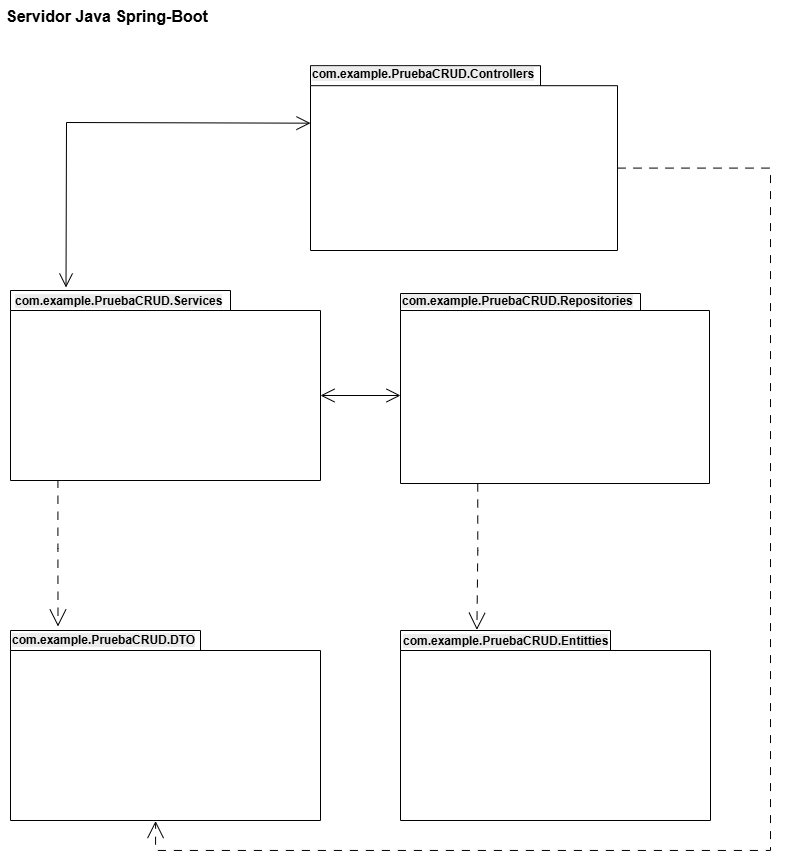
\includegraphics[width=0.8\textwidth]{Clases/DCG.png}
		\caption{Diagrama de la Estructura General del Servidor Java.}
		\label{fig:DCG}
	\end{center}
\end{figure}

A continuación, se presentan los diagramas de cada clase dentro de los paquetes explicados anteriormente.

\newpage
\subsubsection{Entidades}
A continuación, en las figuras \ref{fig:DCERed}, \ref{fig:DE1}, \ref{fig:DE2} y \ref{fig:DE3}, se mostrará más a detalle el contenido que tiene cada uno de los paquetes ilustrados anteriormente. Como primera parte, se muestran las clases que están dentro del paquete \\ `com.example.PruebaCRUD.Entities`. En este diagrama se muestran las relaciones internas entre las clases dentro del paquete ya mencionado.

\begin{figure}[htbp!]
	\begin{center}
		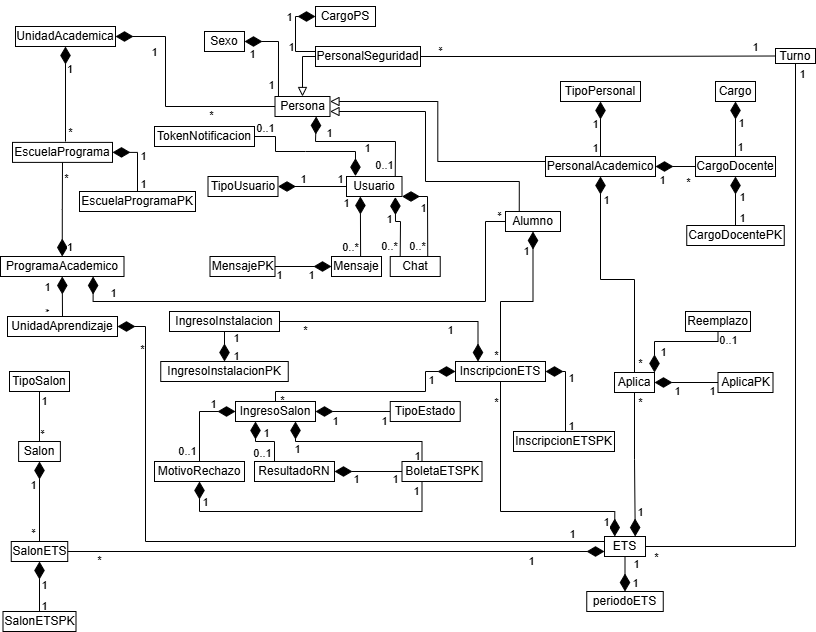
\includegraphics[width=0.8\textwidth]{Clases/DCE Reducido.png}
		\caption{Diagrama de clases general de las entidades del servidor.}
		\label{fig:DCERed}
	\end{center}
\end{figure}

 En este primer diagrama, las clases se muestran sin sus propiedades para una mejor visualización, sin embargo, en las imágenes posteriores se detalla más a profundidad las propiedades de cada una de estas clases.

\newpage

\begin{figure}[htbp!]
	\begin{center}
		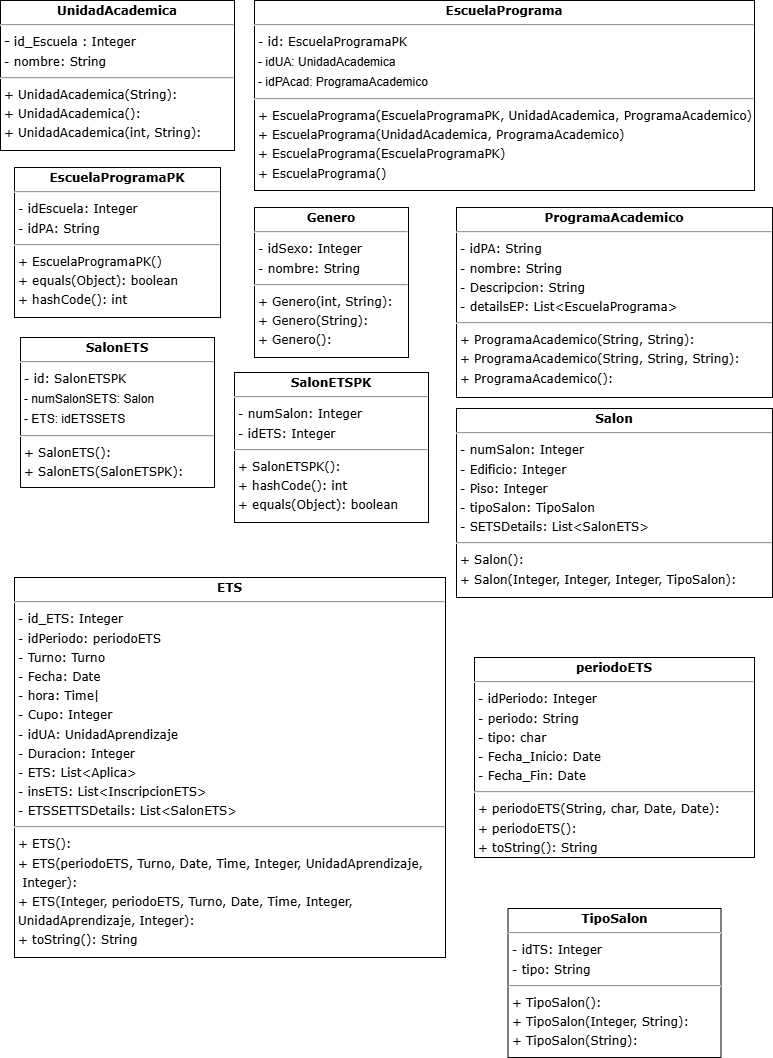
\includegraphics[width=0.8\textwidth]{Clases/EntidadesP1.png}
		\caption{Diagrama de clases de las entidades del servidor parte 1.}
		\label{fig:DE1}
	\end{center}
\end{figure}
\newpage

\begin{figure}[htbp!]
	\begin{center}
		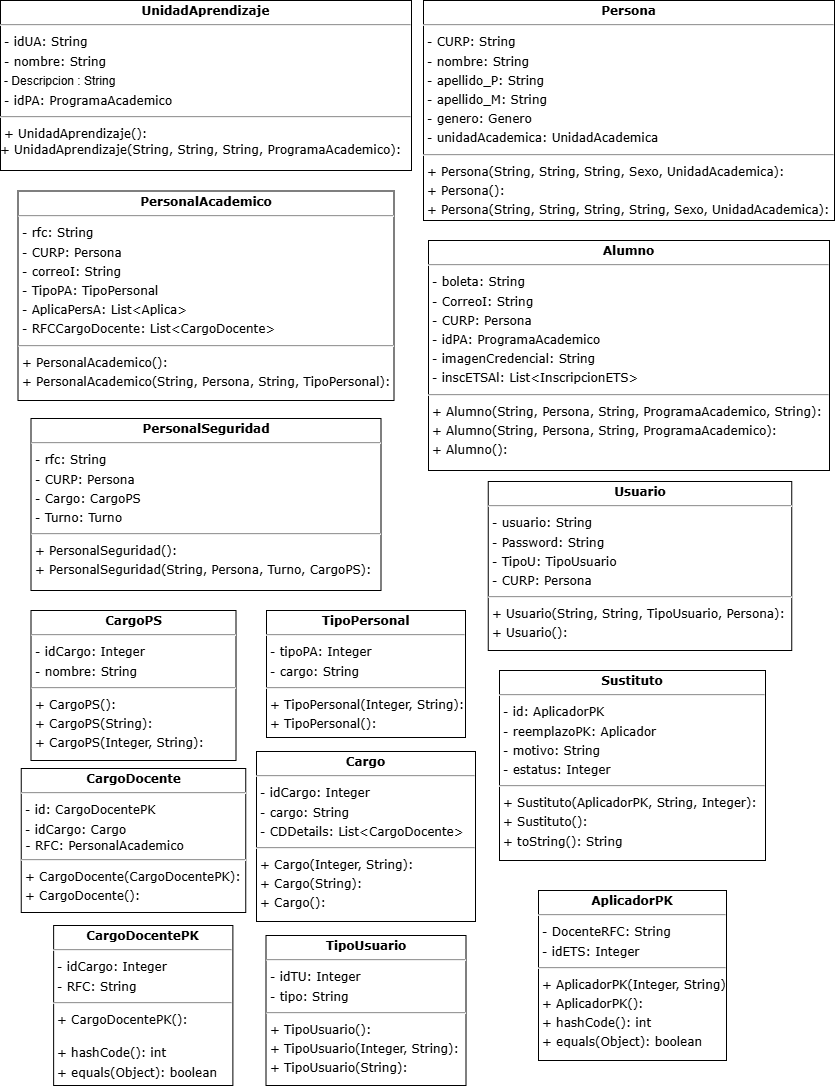
\includegraphics[width=0.8\textwidth]{Clases/EntidadesP2.png}
		\caption{Diagrama de clases de las entidades del servidor parte 2.}
		\label{fig:DE2}
	\end{center}
\end{figure}
\newpage

\begin{figure}[htbp!]
	\begin{center}
		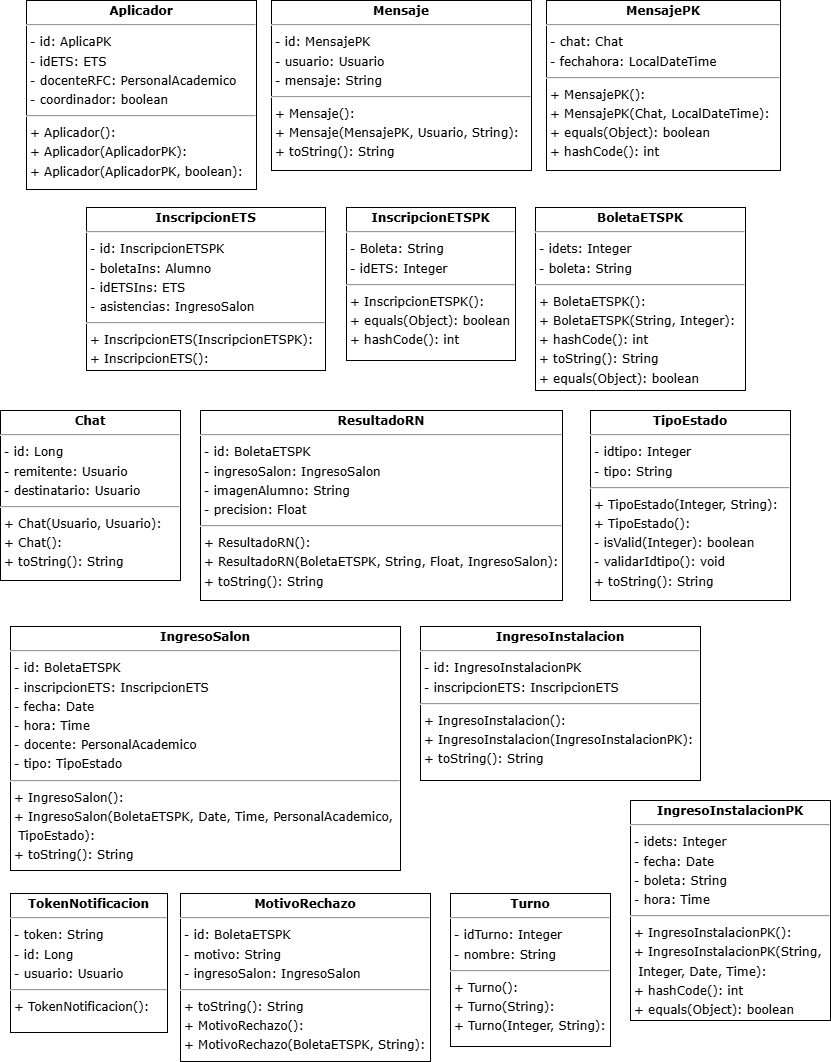
\includegraphics[width=0.8\textwidth]{Clases/EntidadesP3.png}
		\caption{Diagrama de clases de las entidades del servidor parte 3.}
		\label{fig:DE3}
	\end{center}
\end{figure}
\newpage
\subsubsection{Controladores}
En la figura \ref{fig:DC1}, \ref{fig:DC2}, \ref{fig:DC3}, \ref{fig:DC4} y \ref{fig:DC5}, se presentan los diagramas de las clases de los controladores junto con sus respectivas propiedades.

\begin{figure}[htbp!]
	\begin{center}
		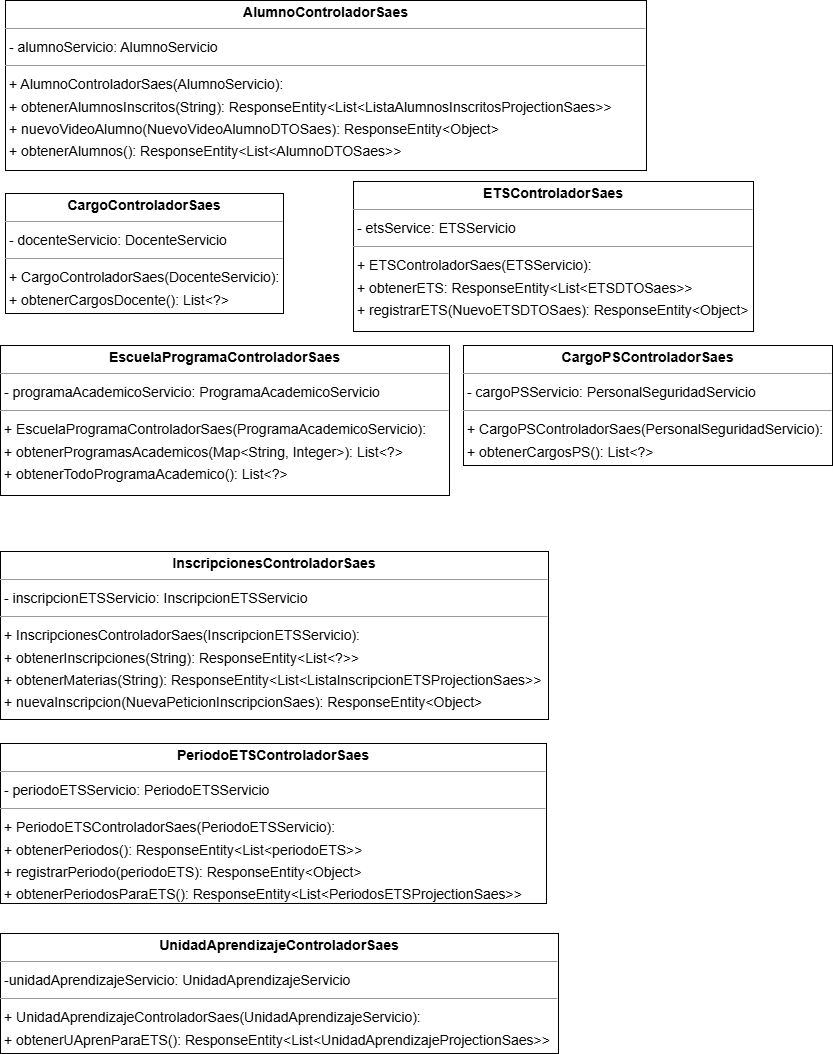
\includegraphics[width=0.7\textwidth]{Clases/Controlador1.png}
		\caption{Diagrama de clases de los controladores del servidor parte 1.}
		\label{fig:DC1}
	\end{center}
\end{figure}

\begin{figure}[htbp!]
	\begin{center}
		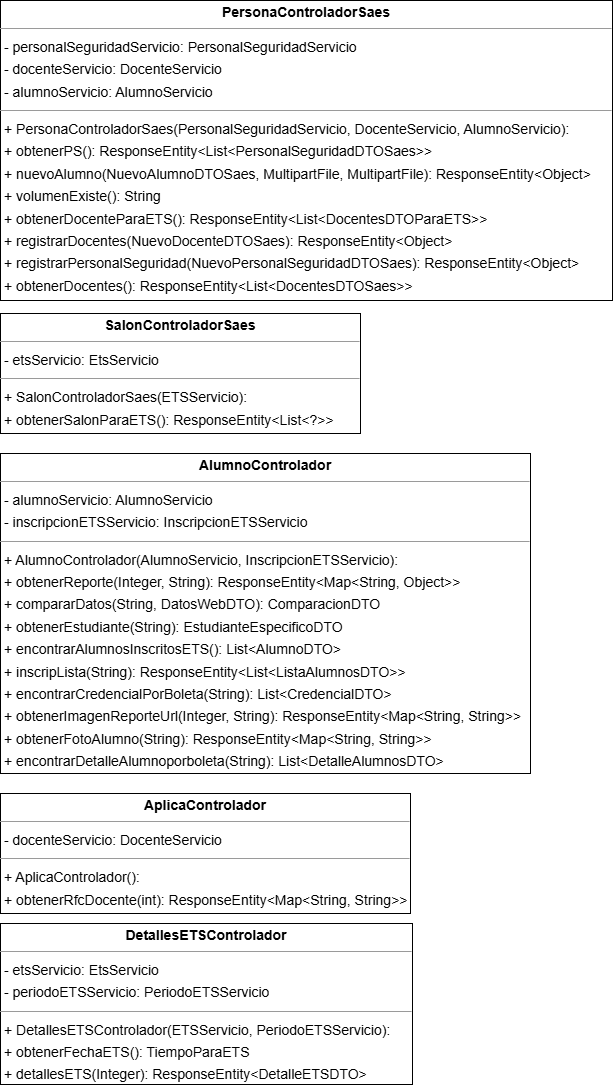
\includegraphics[width=0.65\textwidth]{Clases/Controlador2.png}
		\caption{Diagrama de clases de los controladores del servidor parte 2.}
		\label{fig:DC2}
	\end{center}
\end{figure}

\begin{figure}[htbp!]
	\begin{center}
		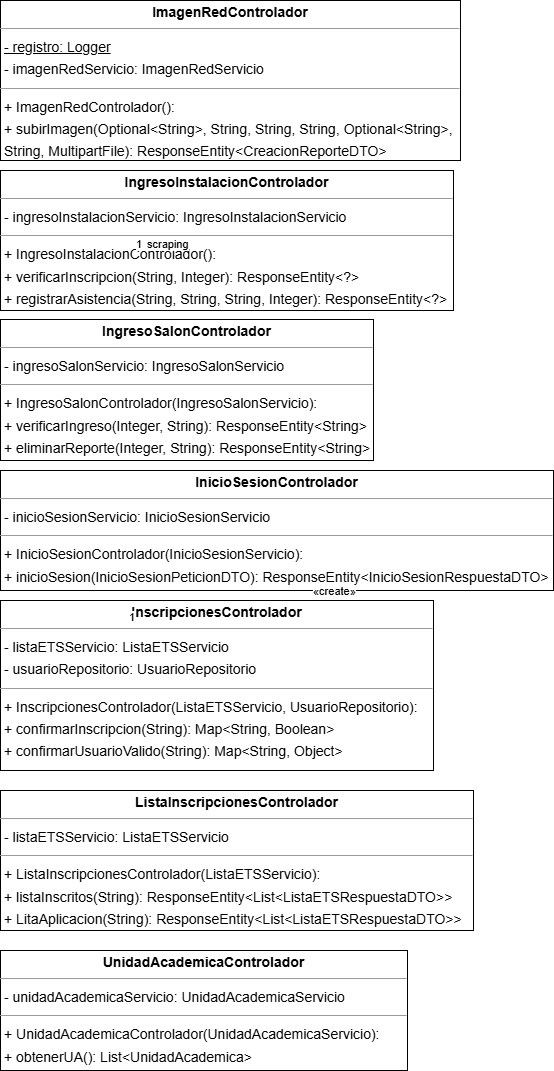
\includegraphics[width=0.6\textwidth]{Clases/Controlador3.png}
		\caption{Diagrama de clases de los controladores del servidor parte 3.}
		\label{fig:DC3}
	\end{center}
\end{figure}

\begin{figure}[htbp!]
	\begin{center}
		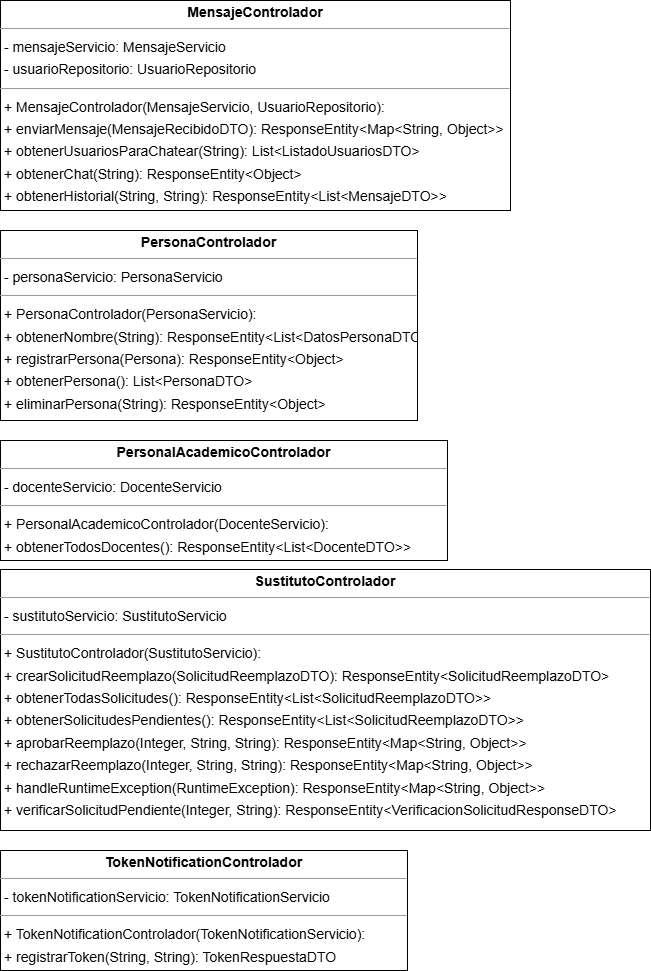
\includegraphics[width=0.75\textwidth]{Clases/Controlador4.png}
		\caption{Diagrama de clases de los controladores del servidor parte 4.}
		\label{fig:DC4}
	\end{center}
\end{figure}

\begin{figure}[htbp!]
	\begin{center}
		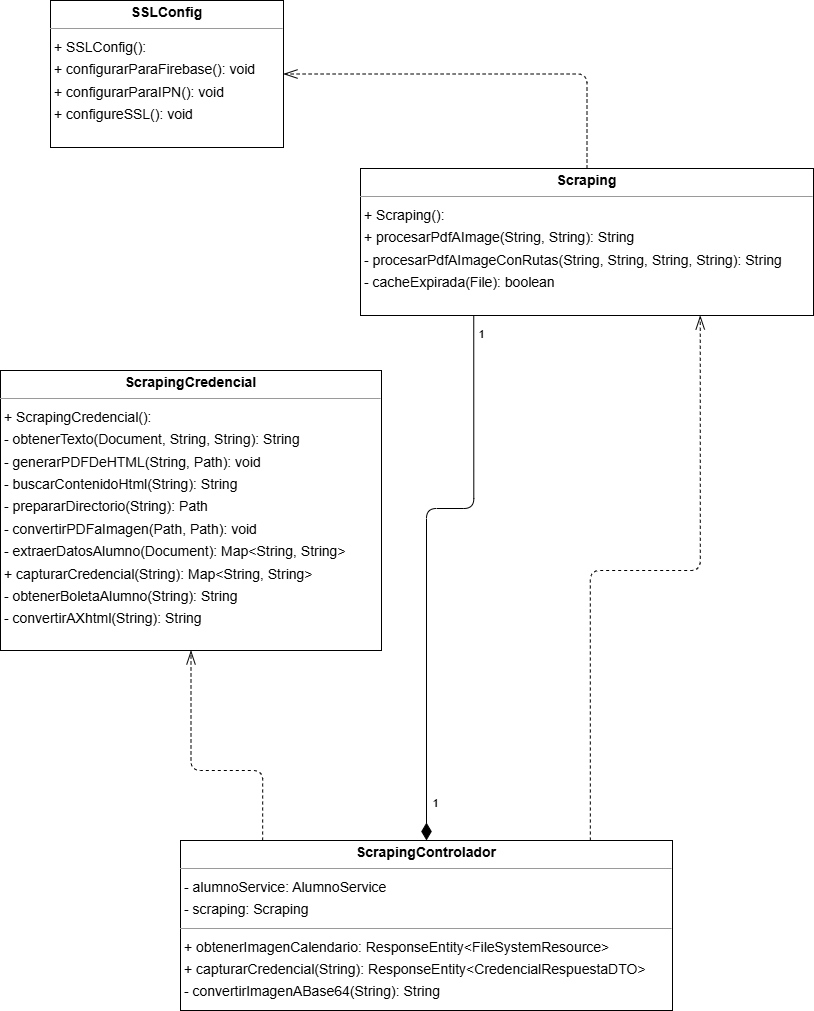
\includegraphics[width=0.9\textwidth]{Clases/Controlador5.png}
		\caption{Diagrama de clases de los controladores del servidor parte 5.}
		\label{fig:DC5}
	\end{center}
\end{figure}
\newpage
\newpage
\subsubsection{Servicios}
A continuación , en las figuras \ref{fig:DS1}, \ref{fig:DS2}, \ref{fig:DS3}, \ref{fig:DS4}, \ref{fig:DS5}, \ref{fig:DS6} y \ref{fig:DS7}, se mostrarán los diagramas de los servicios que conforman al servidor, es decir, los que contienen la lógica del negocio de todo nuestro sistema. A su vez, se mostrarán las propiedades de cada uno de estas clases, es decir, las variables y los métodos que conforman a cada clase.

\begin{figure}[htbp!]
	\begin{center}
		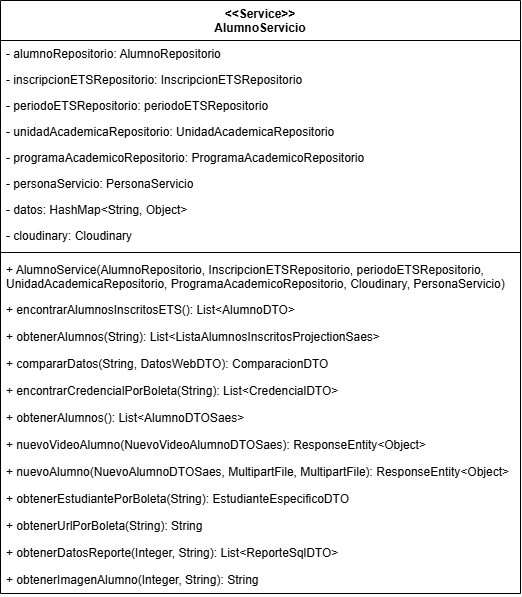
\includegraphics[width=0.8\textwidth]{Clases/Servicio1.png}
		\caption{Diagrama de clases de los servicios del servidor parte 1.}
		\label{fig:DS1}
	\end{center}
\end{figure}

\begin{figure}[htbp!]
	\begin{center}
		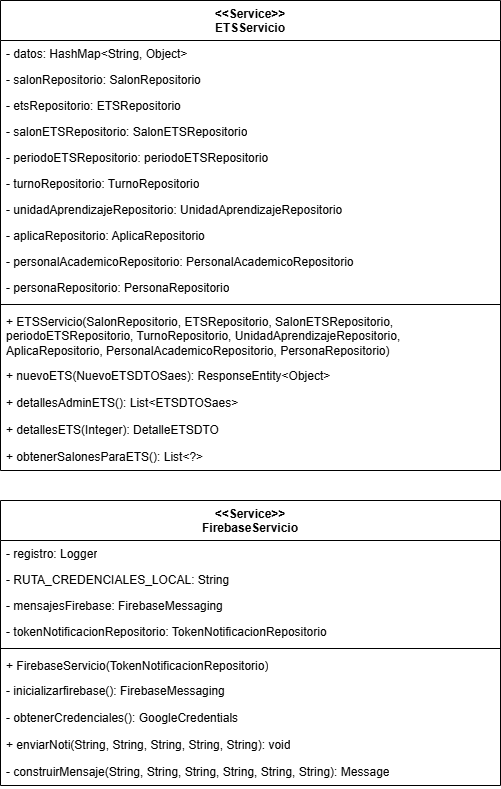
\includegraphics[width=0.7\textwidth]{Clases/Servicio2.png}
		\caption{Diagrama de clases de los servicios del servidor parte 2.}
		\label{fig:DS2}
	\end{center}
\end{figure}


\begin{figure}[htbp!]
	\begin{center}
		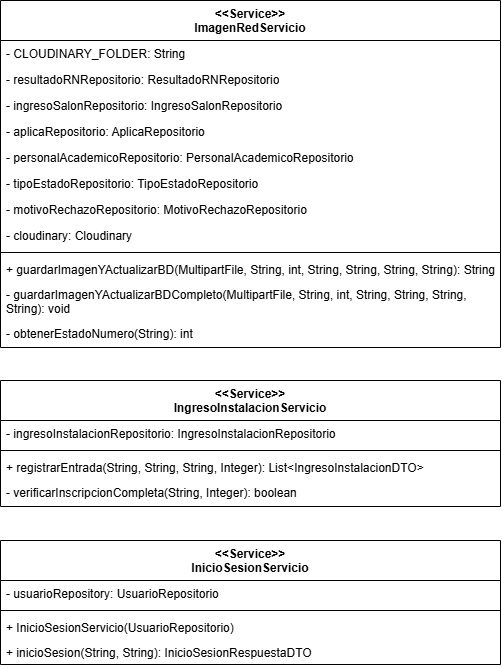
\includegraphics[width=0.8\textwidth]{Clases/Servicio3.png}
		\caption{Diagrama de clases de los servicios del servidor parte 3.}
		\label{fig:DS3}
	\end{center}
\end{figure}

\begin{figure}[htbp!]
	\begin{center}
		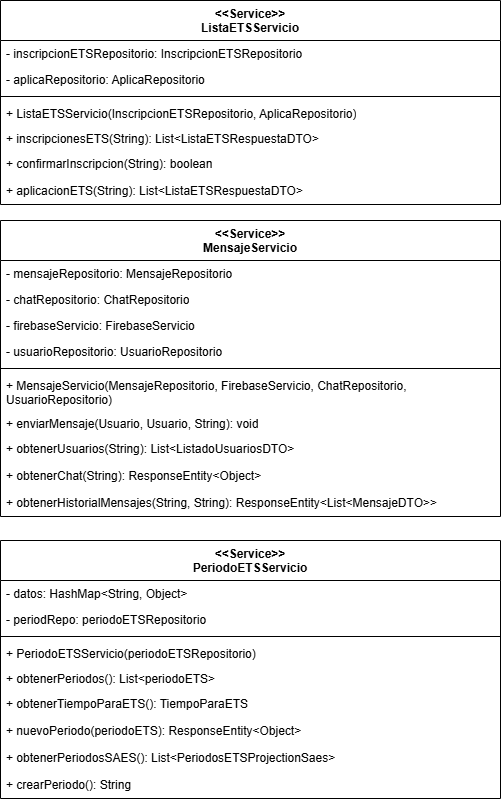
\includegraphics[width=0.7\textwidth]{Clases/Servicio4.png}
		\caption{Diagrama de clases de los servicios del servidor parte 4.}
		\label{fig:DS4}
	\end{center}
\end{figure}

\begin{figure}[htbp!]
	\begin{center}
		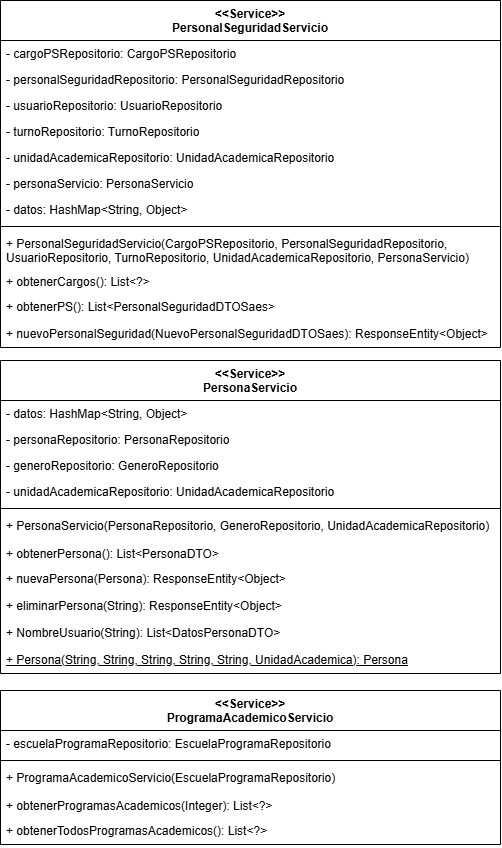
\includegraphics[width=0.7\textwidth]{Clases/Servicio5.png}
		\caption{Diagrama de clases de los servicios del servidor parte 5.}
		\label{fig:DS5}
	\end{center}
\end{figure}

\begin{figure}[htbp!]
	\begin{center}
		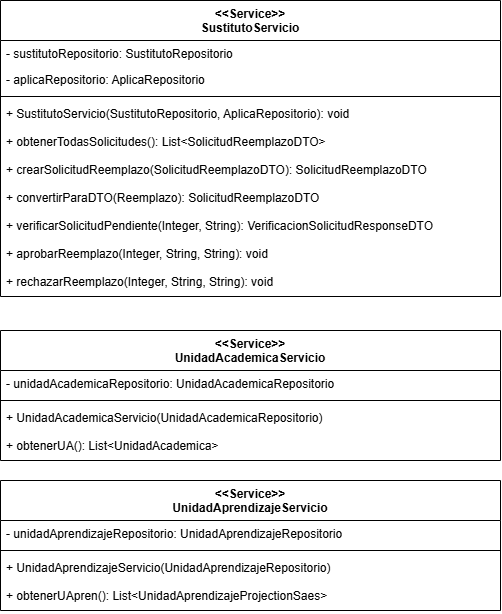
\includegraphics[width=0.8\textwidth]{Clases/Servicio6.png}
		\caption{Diagrama de clases de los servicios del servidor parte 6.}
		\label{fig:DS6}
	\end{center}
\end{figure}

\begin{figure}[htbp!]
	\begin{center}
		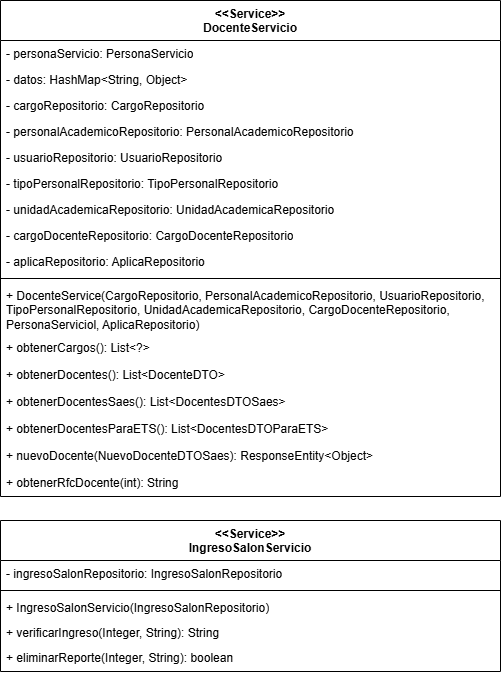
\includegraphics[width=0.8\textwidth]{Clases/Servicio7.png}
		\caption{Diagrama de clases de los servicios del servidor parte 7.}
		\label{fig:DS7}
	\end{center}
\end{figure}

\begin{figure}[htbp!]
	\begin{center}
		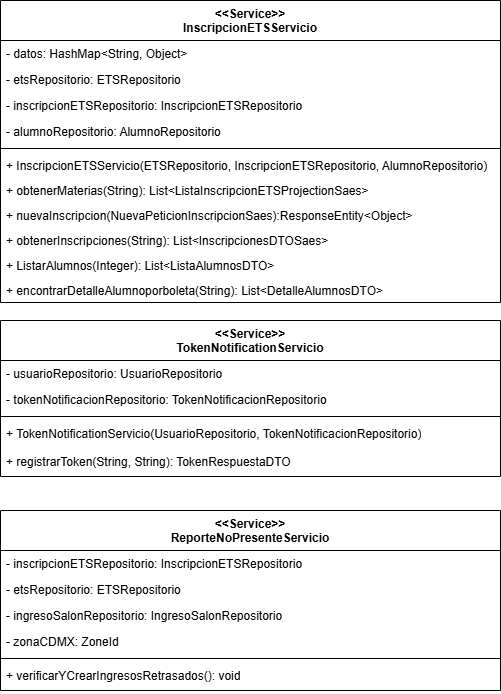
\includegraphics[width=0.8\textwidth]{Clases/Servicio8.png}
		\caption{Diagrama de clases de los servicios del servidor parte 8.}
		\label{fig:DS8}
	\end{center}
\end{figure}
\newpage
\subsubsection{Repositorios}
Ahora, en las figuras \ref{fig:DR1} y \ref{fig:DR2}, se mostrará más a detalle las propiedades y los métodos de cada una de las clases de tipo repositorio que se encuentran dentro del servidor.

\begin{figure}[htbp!]
	\begin{center}
		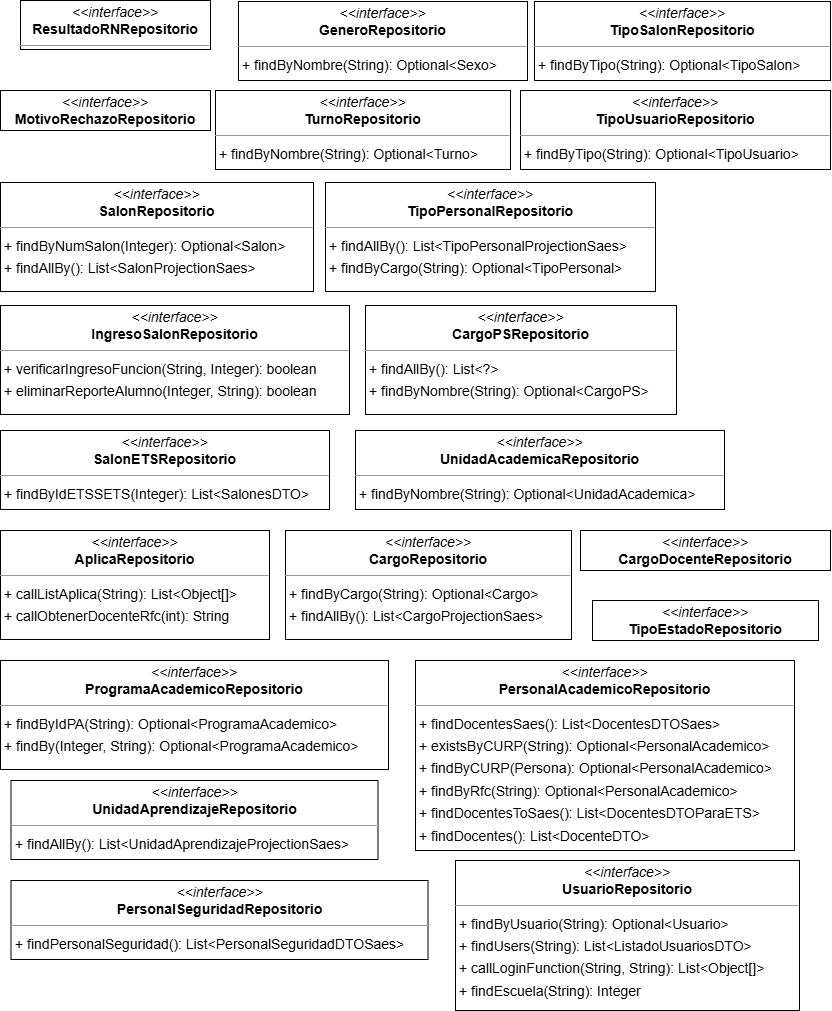
\includegraphics[width=0.8\textwidth]{Clases/Repo1.png}
		\caption{Diagrama de clases de los repositorios del servidor parte 1.}
		\label{fig:DR1}
	\end{center}
\end{figure}

\begin{figure}[htbp!]
	\begin{center}
		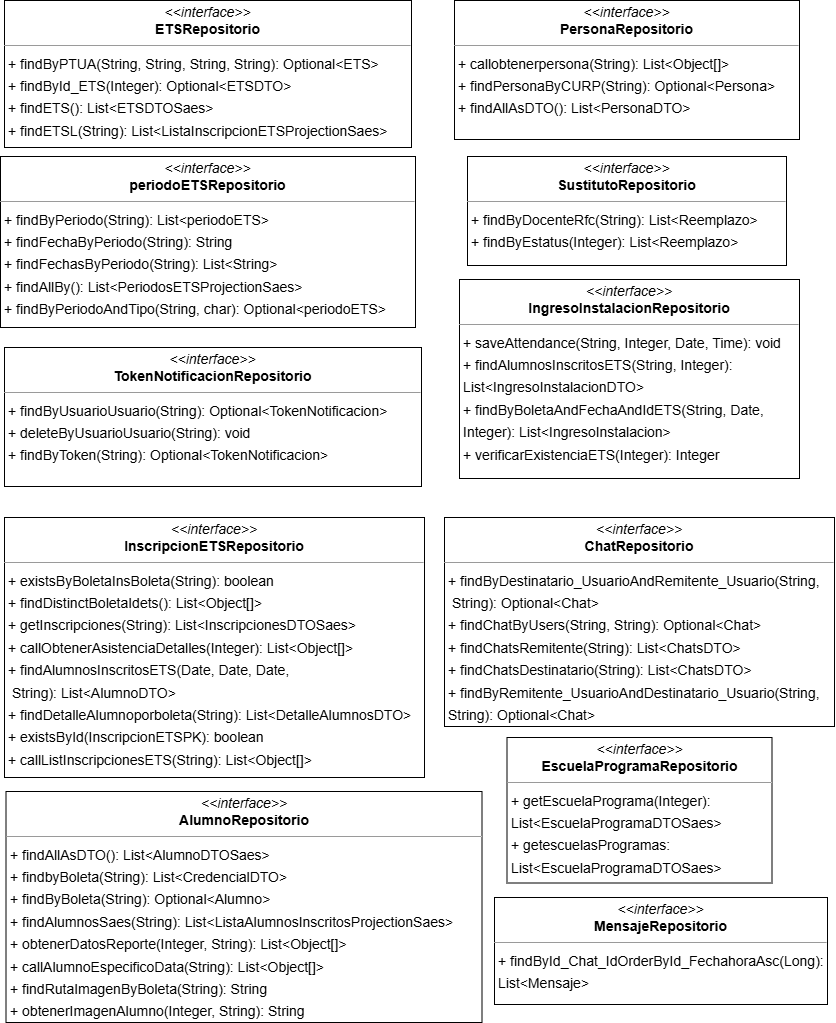
\includegraphics[width=0.8\textwidth]{Clases/Repo2.png}
		\caption{Diagrama de clases de los repositorios del servidor parte 2.}
		\label{fig:DR2}
	\end{center}
\end{figure}
\newpage
\subsubsection{Objetos de Transferencia de datos (DTO)}
Por última parte, en las figuras , tenemos a las clases DTO. Estas clases, como se mencionó anteriormente, son utilizadas por las clases de tipo repositorio, servicio y controlador, por lo que son una pieza clave dentro del proyecto.


\begin{figure}[htbp!]
	\begin{center}
		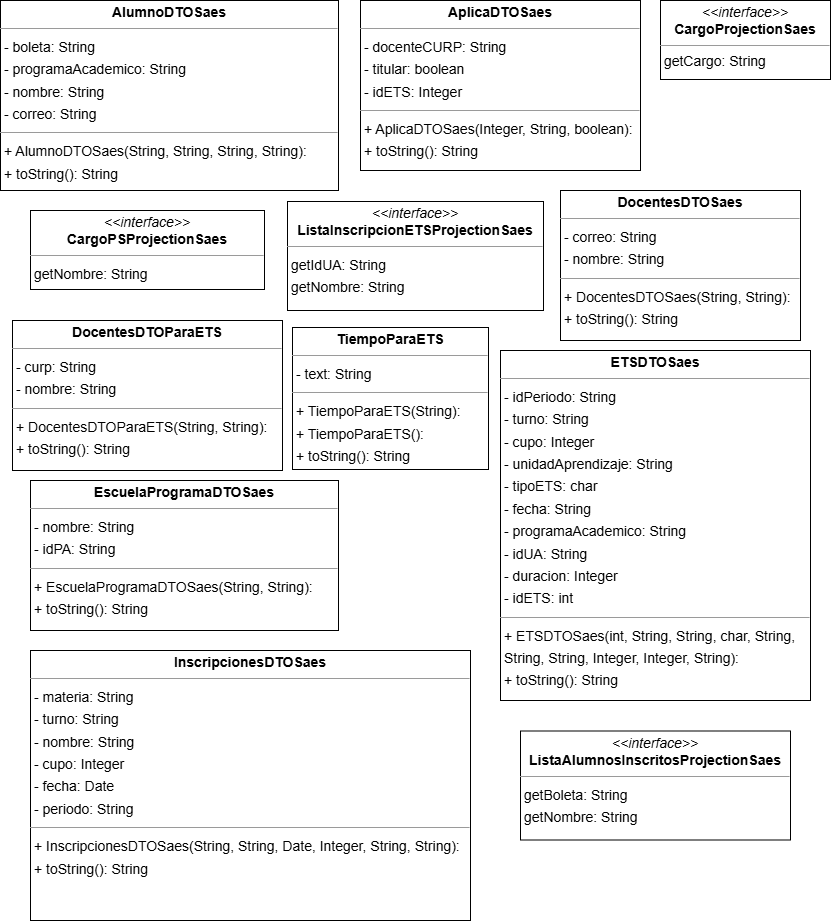
\includegraphics[width=0.85\textwidth]{Clases/DTO1.png}
		\caption{Diagrama de clases de los DTO del servidor parte 1.}
		\label{fig:DTO1}
	\end{center}
\end{figure}

\begin{figure}[htbp!]
	\begin{center}
		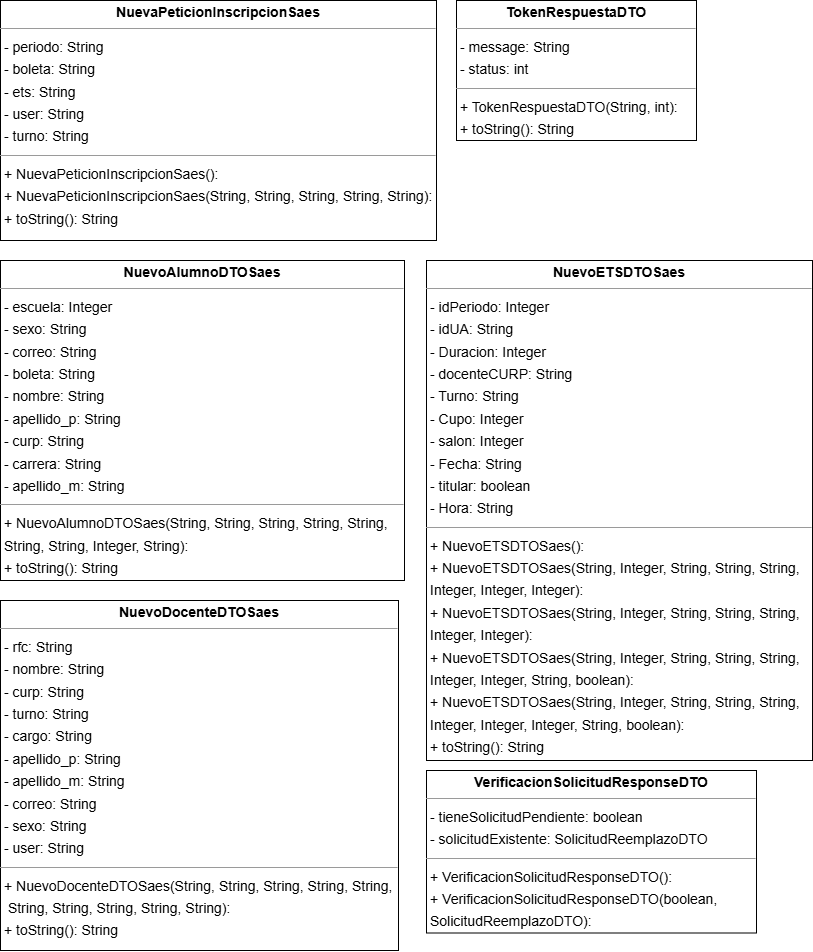
\includegraphics[width=0.9\textwidth]{Clases/DTO2.png}
		\caption{Diagrama de clases de los DTO del servidor parte 2.}
		\label{fig:DTO2}
	\end{center}
\end{figure}

\begin{figure}[htbp!]
	\begin{center}
		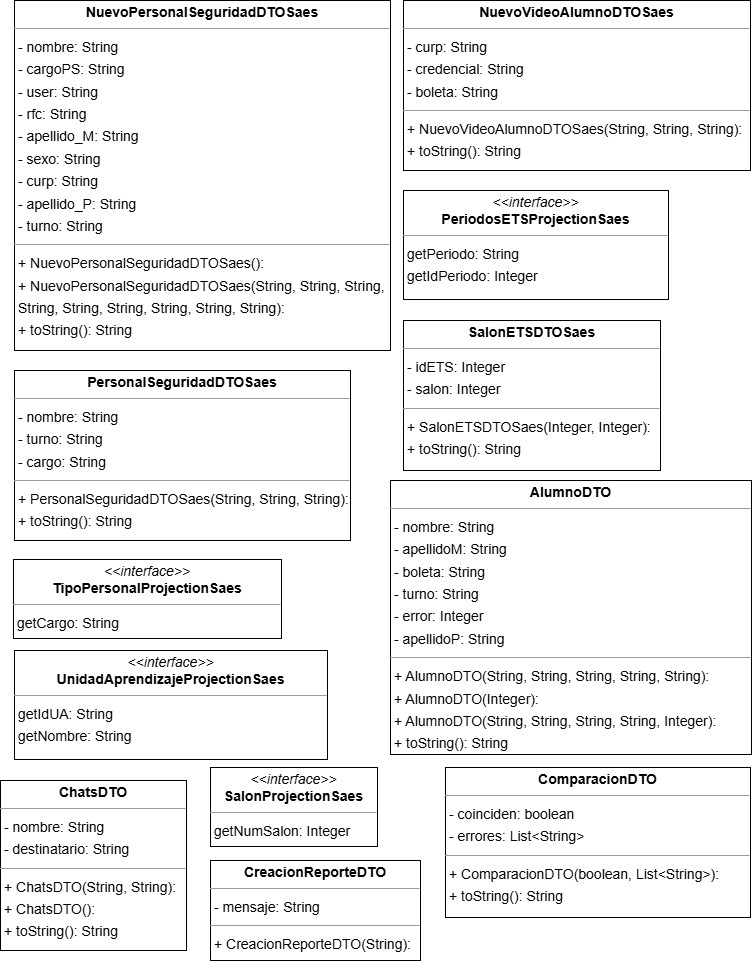
\includegraphics[width=0.9\textwidth]{Clases/DTO3.png}
		\caption{Diagrama de clases de los DTO del servidor parte 3.}
		\label{fig:DTO3}
	\end{center}
\end{figure}

\begin{figure}[htbp!]
	\begin{center}
		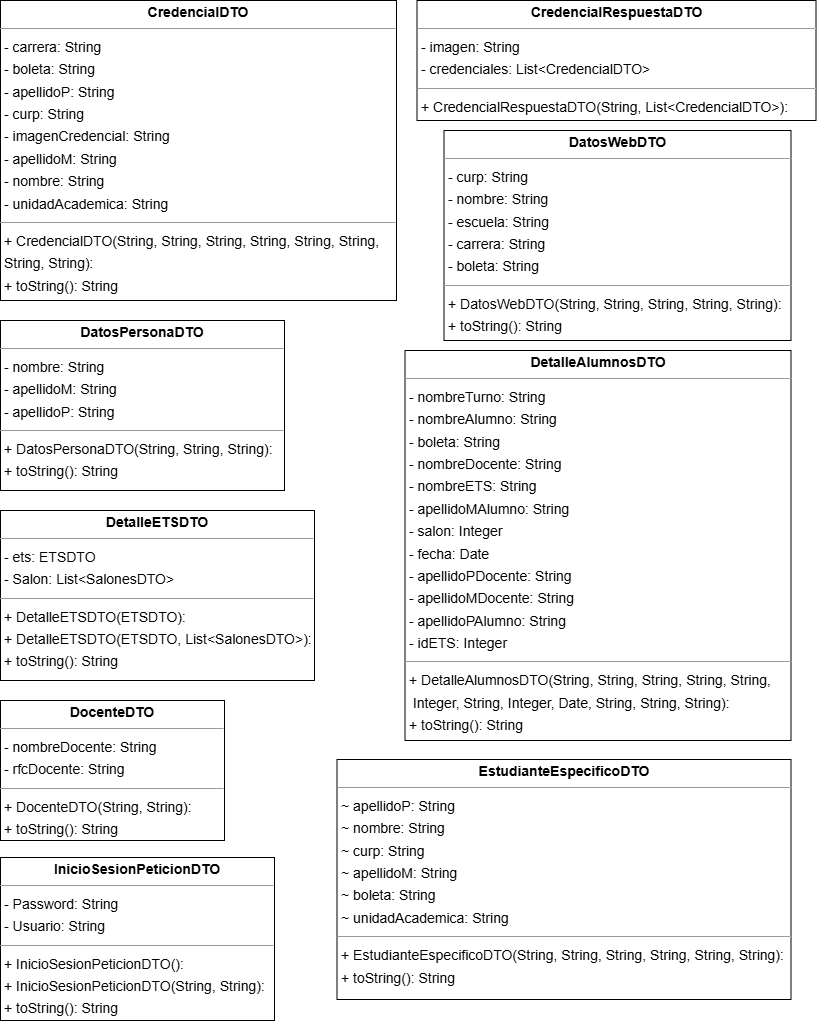
\includegraphics[width=0.9\textwidth]{Clases/DTO4.png}
		\caption{Diagrama de clases de los DTO del servidor parte 4.}
		\label{fig:DTO4}
	\end{center}
\end{figure}

\begin{figure}[htbp!]
	\begin{center}
		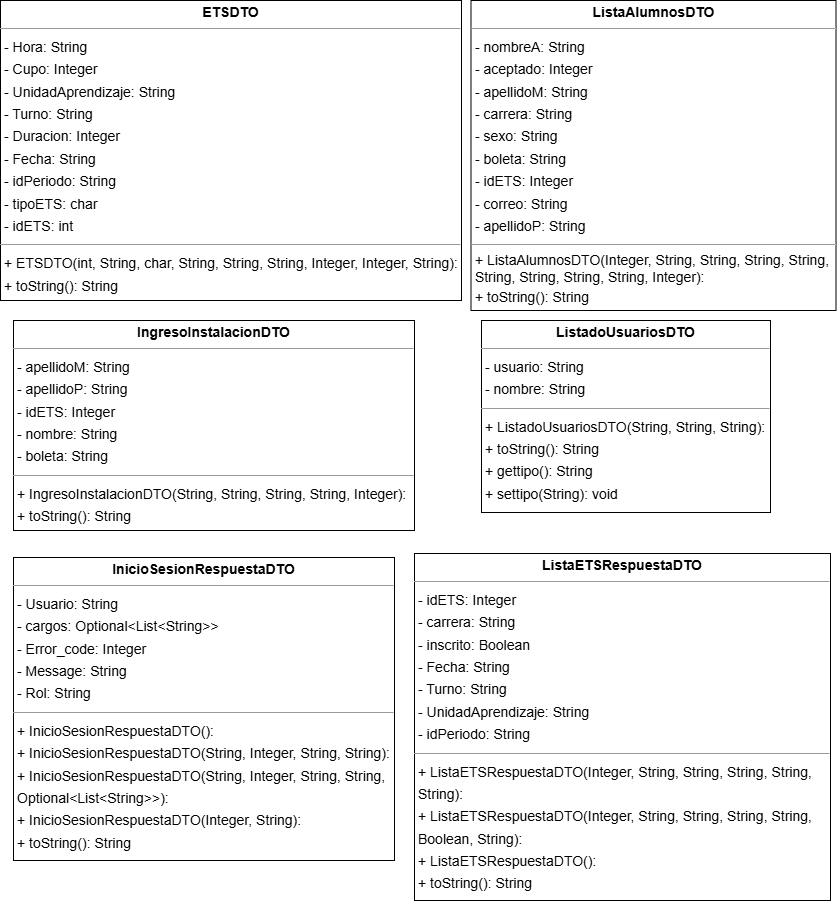
\includegraphics[width=0.9\textwidth]{Clases/DTO5.png}
		\caption{Diagrama de clases de los DTO del servidor parte 5.}
		\label{fig:DTO5}
	\end{center}
\end{figure}

\begin{figure}[htbp!]
	\begin{center}
		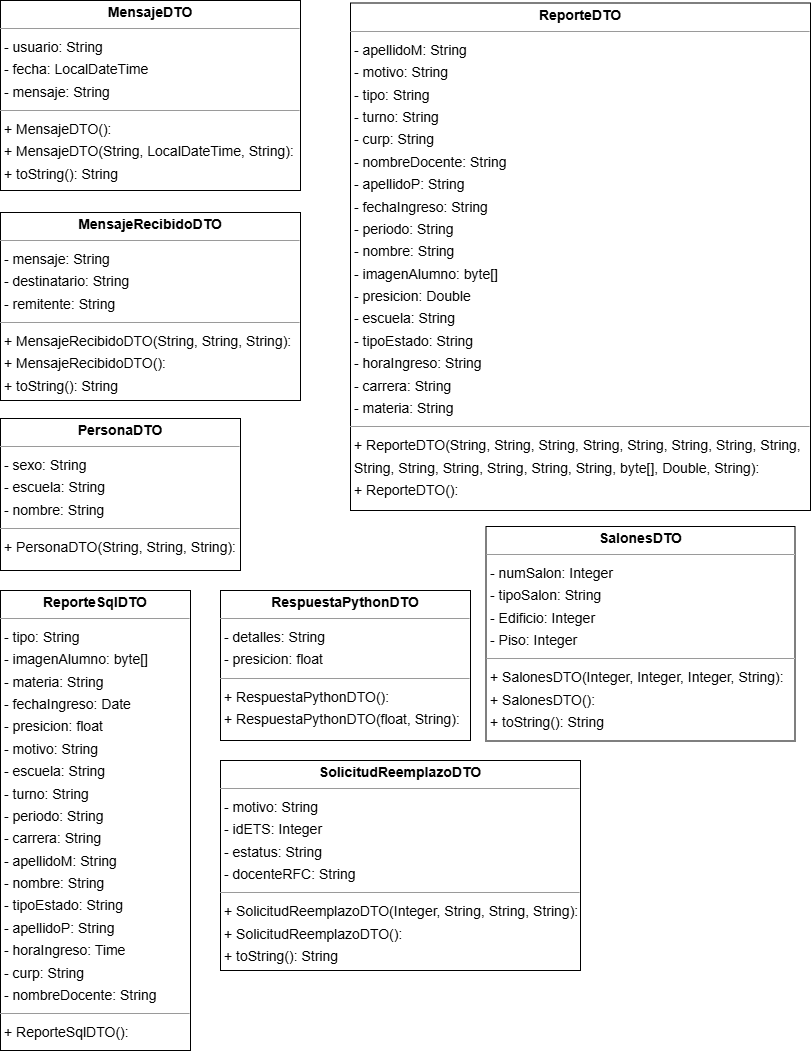
\includegraphics[width=0.9\textwidth]{Clases/DTO6.png}
		\caption{Diagrama de clases de los DTO del servidor parte 6.}
		\label{fig:DTO6}
	\end{center}
\end{figure}
\newpage